\chapter{Guided Transcoding}

\Glsfirst{gt} aims to get around some of the problems presented in the earlier models of adaptive streaming (see \cref{sec:adaptive-streaming}). Instead of working with full encodings of the \gls{lq} representations, we generate \glsfirst{si}\glsunset{si} which is cheaper to store, and then use our highest-resolution video together with the \gls{si} to quickly regenerate the sequences when needed.

"Quick" is this case means that the computational complexity of the regeneration is comparable to that of regular decoding, several orders of magnitude faster than encoding. Because the process is fast -- it can be done in real-time under certain conditions -- we can keep our lower-resolution videos stored only as side-information, and regenerate the full sequence on-demand when requested, thus achieving what is generally not possible in the \gls{jit} transcoding scheme.

So \gls{gt} achieves the virtues of both upfront and \gls{jit} transcoding; we save space by allowing us not to store full encodings of every resolution, but the process is fast so we can generate content on short notice. Guided transcoding can also be seen as a reversal of \gls{svc} in that we save the \gls{hq} video and use that to regenerate \gls{lq} representations, instead of the other way around with a base layer and enhancement layers.

\section{Pruning}
\label{sec:pruning}
Our first model for generating \gls{si} is referred to as \textit{pruning} and was first described in~\cite{Van_Wallendael}. Pruning a bitstream means passing it through a modified decoder that removes transform coefficients and replaces them with sparse dummy matrices that are cheaper to encode. What we are left with is the \textit{mode information}; the frame partitionings and prediction modes chosen for each block, together with motion vectors for every inter coded block.

See \cref{fig:gt-pruning} for a pruning scenario with two lower resolutions. We generate \gls{lq} encodings just like in a simulcast case, prune them and then store the pruned bitstreams to save space. The blocks on the left of the dashed line represent the steps that are performed without time constraints. At a later stage, we use the mode information to recreate the transform coefficients and give a perfect reconstruction of our pruned video. The vertical dots represent repetition. We show two \gls{lq} representations, but the idea can easily be expanded two an arbitrary amount of representations.

To achieve this, we replicate the process that was used to create the \gls{lq} video in the first place. The \gls{hq} bitstream is decoded and downscaled and its pixel data is encoded. Because we have all partitionings and mode decisions stored in the \gls{si}, the process is now much less complex. Even without the \gls{si}, we could encode the downscaled \gls{hq} video and get our \gls{lq} bitstream back. Encoding the same video twice leads the encoder to make all the same mode decisions to create the same bitstream. What that \gls{si} allows us to do is to create the \gls{lq} encoding without having to calculate all the encoder decisions. This is why it is so much faster, the \gls{si} \textit{guides} the encoding process, thus giving the method its name.

\begin{figure}
    \centering
    %\includegraphics[scale=1.1]{pictures/rusert/guided-transcoding}
    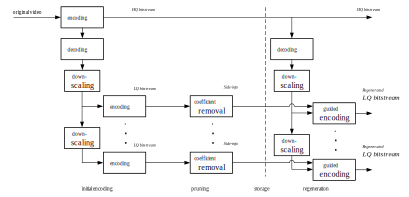
\includegraphics[scale=0.8]{pictures/visio/pruning}
    \caption{Guided transcoding in the pruning scenario}
    \label{fig:gt-pruning}
\end{figure}


\subsection{Generating Side-Information}
%As can be seen in \cref{fig:gt-pruning}, pruning \gls{gt} shares many similarities with the \gls{jit} transcoding scheme presented in \cref{subsec:jit-transcoding}.

Because we won't have access to the original video when regenerating sequences -- it is generally discarded after being used to create the \gls{hq} bitstream, and takes far too much space to store long term -- we treat our \gls{hq} bitstream as an "original" and transcode it to generate \gls{lq} representations.

That is, we decode the \gls{hq} bitstream, downscale it to each desired \gls{lq} resolution and re-encode. Downscaling is performed by passing a decoded video to a downscaler program. This decreases the number of total pixels in the image, lowering its quality and file size while still preserving the overall "look" of each frame. To achieve this, groups of pixels are mapped to single values. Downscaling by a factor of 2 means that each $2 \times 2$ block is replaced by a single pixel. The downscaler looks at a number of adjacent values in the input and calculates a weighted average that it assigns to the pixel value in the output video. Each of the three components in a color image are downscaled separately and the subsampling ratio (see \cref{subsec:subsampling}) is always preserved.

We pass the \gls{lq} representation to the pruner and then store the \gls{si} instead of the full encoding. The pruned bitstream is still decodable, but because all transform coefficients have been removed -- most of them set to 0 -- the video will look far from normal. The screen shows contours of objects, with what looks like very heavy-motion blur, and colors distorted toward pink and purple (see \cref{fig:pruned-frame}).

Because we transcode an already degraded bitstream to generate the \gls{lq} representation -- the \gls{hq} representation is a lossy encoding of the original -- we introduce generation loss. This requires us encode the \gls{lq} bitstreams at a higher bit rate than we would in the simulcast scenario, to achieve the same picture quality.

\begin{figure}
    \centering
    \includegraphics[scale=0.5]{pictures/yuv-player-captures/basketball_drive_fp_640x360_50_dec_38}
    \caption{A decoded frame from a pruned bitstream}
    \label{fig:pruned-frame}
\end{figure}

\subsection{Regenerating a Pruned Sequence}

As mentioned, regenerating a pruned bitstream shares many similarities with regular encoding. The main differences is that we now have two input files instead of one.

The higher-resolution video must be in decoding order, meaning that the frames are output in the order in which they were encoded, not in the order they are meant to be displayed. Non-sequential GOP structures cause the decoder to buffer certain images, use them for predictions, and then output them later when it is their turn to be displayed. We suspend this buffering using a specialized decoder to allow the \gls{hq} video to sync up with the \gls{si}, which is in encoded form, and thus naturally in decoding order.

Regenerating the pruned video means encoding the pixel data from the \gls{hq} representation using the mode information from the \gls{si} to steer the process. Both the pixels and the mode info are the same as were used generate our \gls{lq} bitstream in the first place, so this process will yield a perfect reconstruction of the sequence.

\subsection{Partial Pruning}
\label{subsec:partial_pruning}
Even with the \gls{si} to guide the transcoding process and speed up the process, depending on the hardware that the guided transcoding is running on, it may still be too complex to perform in real-time. This is why we introduced the concept of \textit{partial pruning}. Instead of removing all transform coefficients from a sequence, we prune only certain frames and thus save complexity in the reconstruction.

Our partial pruning scheme is based on temporal layers, and we designate different \textit{pruning levels} based on which layers are excluded from the pruning. Partial pruning level 1 means that the highest temporal layer is excluded, level 2 excludes the top two layers, and so on. The higher temporal layers consist of P-frames and B-frames (see \cref{subsec:gops-and-temporal-layers}). They reference other frames for their predictions, and will generally contain fewer transform coefficients. Thus, our expectation is that partial pruning level 1 or 2 will have a minimal effect of bit rate while still saving a significant amount of complexity in the reconstruction. Then the effectiveness tapers off as we increase the pruning level.

A partially pruned frame at level 3 can be seen in \cref{fig:partially-pruned-frame}. It still has the characteristic look of pruning, but certain pixel values are now retained to hint at the appearance of the original frame.

\begin{figure}
    \centering
    \includegraphics[scale=0.5]{pictures/yuv-player-captures/basketball_drive_pp_l3_640x360_50_dec_38}
    \caption{A decoded frame from a partially pruned bitstream}
    \label{fig:partially-pruned-frame}
\end{figure}


\section{Deflation}
A second guided transcoding idea is introduced in this thesis and we call it \textit{deflation}. In this scenario we encode our \gls{lq} representations directly from the original video, so there is no transcoding loss like for pruning. See \cref{fig:gt-deflation}.

\begin{figure}
    \centering
    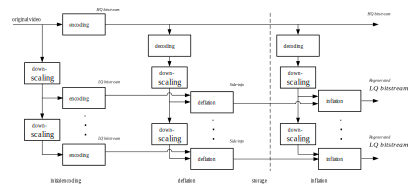
\includegraphics[scale=0.8]{pictures/visio/deflation}
    \caption{Guided transcoding in the deflation scenario}
    \label{fig:gt-deflation}
\end{figure}

\subsection{Generating Side-Information}
%We downscale the original to each desired resolution and encode \gls{lq} the representations. These are then passed to a deflator together with the \gls{hq} video.

To deflate a video, we use two inputs. The mode information from the \gls{lq} bitstream together with the pixel data from the \gls{hq} video are used to generate predictions and calculate a residual. This residual is frequency transformed and quantized (see \cref{subsec:quantization}) and then subtracted from the coefficients in the \gls{lq} bitstream. Because the \gls{hq} and \gls{lq} videos emanate from the same original, this difference is expected to be small and therefore cheap to encode.

In fact, some transform block in the deflated bitstream are likely to be all-zeros, and \gls{hevc} does not allow that. So we identify all matrices of the form shown in \cref{eq:n0-matrix-deflation} and increase the $k$ coefficient by one to create a compliant bitstream.

This scheme maps the highest possible value -- \texttt{SHRT{\_}MAX} because we are storing transform coefficients in variables of type \texttt{short} -- and the one just below it to the same position, potentially introducing a small distortion. However, most values will actually residue around 0, especially this lowest-frequency component, and this distortion has never appeared once in any of our simulations.

\begin{equation}
\label{eq:n0-matrix-deflation}
\begin{pmatrix}
	k & 0 & \cdots & 0 \\
	0 & 0 & \cdots & 0 \\
	\vdots  & \vdots  & \ddots & \vdots \\
	0 & 0 & \cdots & 0
\end{pmatrix} , \quad 0 \leq k < \texttt{SHRT{\_}MAX}
\end{equation}

\subsection{Regenerating a Deflated Sequence}
Reversing the deflation is called \textit{inflation} and replicates many of the steps of the deflation process. We reverse the last step from the deflation by looking for matrices of the form \cref{eq:n0-matrix-deflation}, but with $k \geq 1$, and subtract one.

Because the mode information from the \gls{lq} is untouched by the deflation, we can once again downscale the \gls{hq} video and generate a residual. After frequency transformation and quantization we re-add the transform coefficients to the deflated bitstream and thus restore our \gls{lq} video. Just like in the pruning scenario, the \gls{si} guides the encoding of the pixels from the \gls{hq} video, so the process is much faster than a full encoding.